% Human-in-the-loop continual learning: the doctor feedback loop, English, compact.
%
% Companion to feedback_loop_tikz.tex, which stays as the Vietnamese original.
% Two differences, both deliberate:
%
%   1. English, for showing outside the thesis document.
%   2. The two planned components (active-learning worklist ordering and
%      confident-learning label screening) are NOT drawn. They were dashed in
%      the original to mark them as future work; a figure meant to show what
%      exists should not spend a third of its width on what does not. Their
%      absence is why this one is shorter.
%
% Every solid box below maps to code that runs and has a test:
%   grade    -> app/inference/{full_grading,grading}.py  (_load_model reads ACTIVE)
%   corr     -> models_db.CorrectionLog (+ submitted_at, batch_id)
%   batch    -> POST /corrections/submit  (routers/feedback.py)
%   build    -> app/feedback/build_dataset.py   (submitted batches only)
%   retrain  -> app/feedback/retrain_head.py    (_freeze_batchnorm + --replay-dir)
%   holdout  -> app/feedback/freeze_holdout.py  (MANIFEST.json, sha256)
%   gate     -> retrain_head.evaluate()
%   approve  -> POST /model/activate
%   registry -> app/feedback/model_registry.py  (ACTIVE pointer, immutable baseline)
%   revert   -> POST /model/revert
%
% Build:  pdflatex feedback_loop_en.tex
\documentclass[border=8pt]{standalone}
\usepackage[T1]{fontenc}
\usepackage{tikz}
\usepackage{lmodern}
\usetikzlibrary{positioning,arrows.meta,fit,backgrounds,calc}
\begin{document}
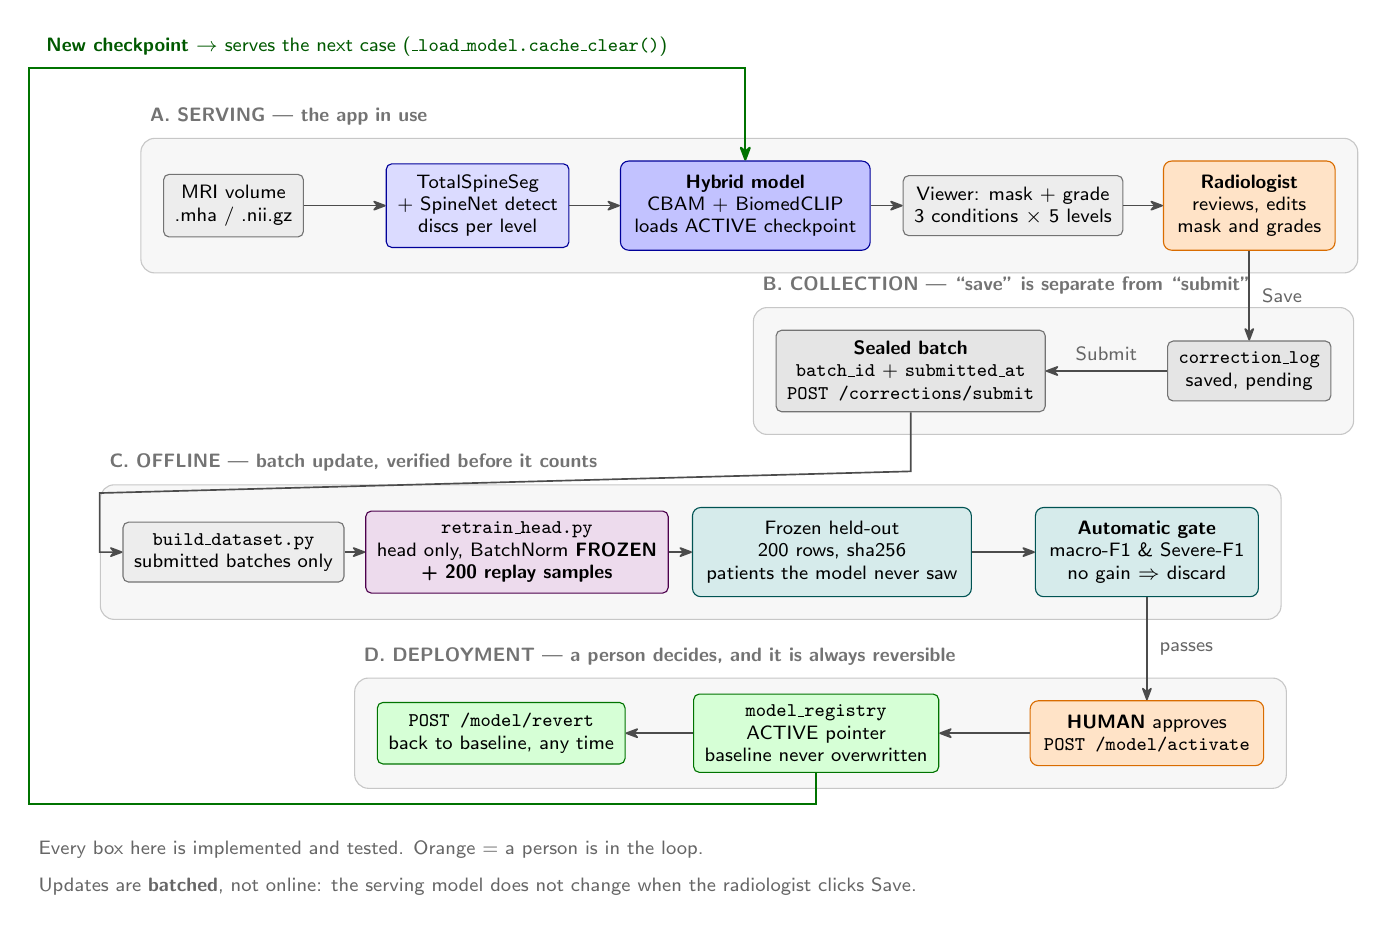
\begin{tikzpicture}[
  font=\sffamily,
  >={Stealth[round]},
  io/.style={rectangle,rounded corners=2pt,draw=black!55,fill=black!7,
             align=center,inner sep=4pt,font=\sffamily\scriptsize},
  net/.style={rectangle,rounded corners=2pt,draw=blue!60!black,fill=blue!14,
              align=center,inner sep=4pt,font=\sffamily\scriptsize},
  model/.style={rectangle,rounded corners=3pt,draw=blue!60!black,fill=blue!24,
                align=center,inner sep=5pt,font=\sffamily\scriptsize},
  human/.style={rectangle,rounded corners=3pt,draw=orange!85!black,fill=orange!22,
                align=center,inner sep=5pt,font=\sffamily\scriptsize},
  data/.style={rectangle,rounded corners=2pt,draw=black!55,fill=black!10,
               align=center,inner sep=4pt,font=\sffamily\scriptsize},
  train/.style={rectangle,rounded corners=2pt,draw=violet!60!black,fill=violet!14,
                align=center,inner sep=4pt,font=\sffamily\scriptsize},
  gate/.style={rectangle,rounded corners=3pt,draw=teal!65!black,fill=teal!16,
               align=center,inner sep=5pt,font=\sffamily\scriptsize},
  deploy/.style={rectangle,rounded corners=2pt,draw=green!45!black,fill=green!16,
                 align=center,inner sep=4pt,font=\sffamily\scriptsize},
  band/.style={rectangle,rounded corners=5pt,draw=black!22,fill=black!3,inner sep=8pt},
  bandlab/.style={font=\sffamily\bfseries\scriptsize,text=black!55,align=left},
  arr/.style={->,semithick,black!70},
  lbl/.style={font=\sffamily\scriptsize,text=black!60,align=center}
]

%% ================= A. SERVING =================
\node[io]    (mri)   at ( 0.0, 2.6) {MRI volume\\\scriptsize .mha / .nii.gz};
\node[net]   (seg)   at ( 3.1, 2.6) {TotalSpineSeg\\+ SpineNet detect\\\scriptsize discs per level};
\node[model] (grade) at ( 6.5, 2.6) {\textbf{Hybrid model}\\CBAM + BiomedCLIP\\\scriptsize loads ACTIVE checkpoint};
\node[io]    (view)  at ( 9.9, 2.6) {Viewer: mask + grade\\\scriptsize 3 conditions $\times$ 5 levels};
\node[human] (doc)   at (12.9, 2.6) {\textbf{Radiologist}\\reviews, edits\\mask and grades};
\foreach \a/\b in {mri/seg, seg/grade, grade/view, view/doc} \draw[arr] (\a) -- (\b);

\begin{scope}[on background layer]
  \node[band,fit=(mri)(doc)] (bandA) {};
\end{scope}
\node[bandlab,anchor=south west] at ([yshift=1pt]bandA.north west)
  {A. SERVING \textmd{---} the app in use};

%% ================= B. COLLECTION =================
\node[data]  (corr)  at (12.9, 0.5) {\texttt{correction\_log}\\\scriptsize saved, pending};
\node[data]  (batch) at ( 8.6, 0.5) {\textbf{Sealed batch}\\\scriptsize \texttt{batch\_id} + \texttt{submitted\_at}\\\scriptsize \texttt{POST /corrections/submit}};
\draw[arr] (doc) -- node[lbl,right=1pt]{Save} (corr);
\draw[arr] (corr) -- node[lbl,above]{Submit} (batch);

\begin{scope}[on background layer]
  \node[band,fit=(batch)(corr)] (bandB) {};
\end{scope}
\node[bandlab,anchor=south west] at ([yshift=1pt]bandB.north west)
  {B. COLLECTION \textmd{---} ``save'' is separate from ``submit''};

%% ================= C. OFFLINE =================
\node[io]    (build) at ( 0.0,-1.8) {\texttt{build\_dataset.py}\\\scriptsize submitted batches only};
\node[train] (retr)  at ( 3.6,-1.8) {\texttt{retrain\_head.py}\\head only, BatchNorm \textbf{FROZEN}\\\textbf{+ 200 replay samples}};
\node[gate]  (hold)  at ( 7.6,-1.8) {Frozen held-out\\\scriptsize 200 rows, sha256\\\scriptsize patients the model never saw};
\node[gate]  (gate)  at (11.6,-1.8) {\textbf{Automatic gate}\\macro-F1 \& Severe-F1\\\scriptsize no gain $\Rightarrow$ discard};
\foreach \a/\b in {build/retr, retr/hold, hold/gate} \draw[arr] (\a) -- (\b);
\draw[arr] (batch.south) -- ++(0,-0.75) -- (-1.7,-1.05)
      -- (-1.7,-1.8) -- (build.west);

\begin{scope}[on background layer]
  \node[band,fit=(build)(gate)] (bandC) {};
\end{scope}
\node[bandlab,anchor=south west] at ([yshift=1pt]bandC.north west)
  {C. OFFLINE \textmd{---} batch update, verified before it counts};

%% ================= D. DEPLOYMENT =================
\node[human] (appr)  at (11.6,-4.1) {\textbf{HUMAN} approves\\\scriptsize \texttt{POST /model/activate}};
\node[deploy](reg)   at ( 7.4,-4.1) {\texttt{model\_registry}\\\scriptsize ACTIVE pointer\\\scriptsize baseline never overwritten};
\node[deploy](rev)   at ( 3.4,-4.1) {\texttt{POST /model/revert}\\\scriptsize back to baseline, any time};
\draw[arr] (gate) -- node[lbl,right=1pt]{passes} (appr);
\draw[arr] (appr) -- (reg);
\draw[arr] (reg)  -- (rev);

\begin{scope}[on background layer]
  \node[band,fit=(rev)(appr)] (bandD) {};
\end{scope}
\node[bandlab,anchor=south west] at ([yshift=1pt]bandD.north west)
  {D. DEPLOYMENT \textmd{---} a person decides, and it is always reversible};

%% ================= the loop closes =================
\draw[arr,green!45!black,thick] (reg.south) -- (7.4,-5.0) -- (-2.6,-5.0)
  -- (-2.6,4.35) -- (6.5,4.35) -- (grade.north);
\node[lbl,text=green!35!black,anchor=west] at (-2.5,4.62)
  {\textbf{New checkpoint} $\rightarrow$ serves the next case \scriptsize(\texttt{\_load\_model.cache\_clear()})};

\node[lbl,anchor=north west] at (-2.6,-5.35)
  {Every box here is implemented and tested. Orange = a person is in the loop.};
\node[lbl,anchor=north west] at (-2.6,-5.82)
  {Updates are \textbf{batched}, not online: the serving model does not change when the radiologist clicks Save.};

\end{tikzpicture}
\end{document}
